% Copyright 2013 Aaron Ecay and Meredith Tamminga
% Available under the Creative Commons BY-SA or GPL v2+ licenses: see
% the file LICENSE for more information

\documentclass{digs-slides}
\usepackage{expex}
\usepackage{multicol}
\usepackage{amssymb}
% \bibliographystyle{linquiry2}

\newcommand{\includegraph}[1]{\mode<beamer>{\input{#1.tikz}}
    \mode<handout>{\input{#1-handout.tikz}}}

\addbibresource{biblio.bib}

\title{Persistence as a diagnostic of grammatical status: The case of Middle English negation}
\author{Aaron Ecay and Meredith Tamminga}
\institute{University of Pennsylvania}
\date{Aug.\ 1, 2013 \\\vspace{0.5em} Diachronic Generative Syntax 15}

\begin{document}

\begin{frame}
    \titlepage
\end{frame}

\section{Introduction}

\subsection*{foo}

\begin{frame}{Introduction}
    \begin{itemize}
      \item Diachronic generative syntax encompasses the analysis both
        of historical grammatical structures and of the processes by
        which they change
      \item Analysis of underlying structures is particularly challenging
        without access to native speakers
    \end{itemize}
\end{frame}

\begin{frame}<beamer>
    \frametitle{Introduction}
    \begin{itemize}
      \item Researchers have made headway by using the Constant Rate
        Effect \parencite{Kroch1989} to infer grammatical
        analyses through quantitative data on historical change
      \item We will propose an independent source of quantitative
        evidence about historical grammatical analyses: clustering
        tendencies across tokens
    \end{itemize}
\end{frame}

\begin{frame}
    \frametitle{Table of contents}
    \tableofcontents{}
\end{frame}

\section{Background: Persistence}

\subsection*{foo}

\begin{frame}{The persistence effect}
	\begin{itemize}
          \item Individual observations of variable phenomena are not independent \parencite{Sankoff:1978}
		\item \textbf{Persistence:} the tendency to repeat the same linguistic option again in natural speech
		\item Inherently interesting phenomenon, but also a useful dependent variable for its reflection of underlying structures
	\end{itemize}
\end{frame}

\begin{frame}{Experimental structural priming}
	\begin{itemize}
		\item Persistence seems to be related to the experimental phenomenon of priming
		\item Extensive structural priming
                  literature \parencite[beginning with][]{Bock:1986}
                  demonstrates that syntactic structures can be primed
		\item For example, use of a double-object construction gives rise to a preference for double-object over prepositional dative
		% nice clean citation for this one? just Bock?
	\end{itemize}
\end{frame}

\begin{frame}{Persistence in written and spoken corpora}
	\begin{itemize}
          \item Early demonstrations of persistence in spoken language include number agreement in Spanish DPs \parencite{Poplack:1980} and passive alternation \parencite{Weiner:1983}
          \item \textcite{Gries:2005} finds that persistence effects in both written and spoken corpora are consistent with experimental results for the same constructions
		\item Linking hypothesis: persistence effects in written historical data reflect priming effects in language production at the time
	\end{itemize}
\end{frame}


\begin{frame}{Structural identity in persistence}
	\begin{itemize}
		\item Tendency to repeat the same linguistic option — repetition reveals sameness
		\item “If the processing of a stimulus affects the processing of another stimulus, then the two stimuli must be related [...] if the relationship between the two stimuli is syntactic, then we can use this relationship as a way of understanding what syntactic information is represented” \parencite[490]{Branigan:1995}
	\end{itemize}
\end{frame}

\begin{frame}{Previous demonstrations of structural identity}
	\begin{itemize}
          \item \textcite{Estival:1985}: different types of passives (lexical vs.\ transformational) each facilitate themselves but not each other
          \item The structural distinction this reflects is maintained in modern syntactic accounts \parencite[e.g.][]{Embick:2004}
	\end{itemize}
        % Code for this graph:
        % > estival.graph(write = TRUE)
        \begin{center}
            \includegraph{figures/estival}
        \end{center}
\end{frame}

\begin{frame}{Previous demonstrations of structural identity in persistence} % priming?
	\begin{itemize}
          \item \textcite{Bock:1990}: Infinitival purpose clauses with
            “to” do not facilitate prepositional datives with “to”
            \begin{itemize}
              \item I brought a book to study
              \item I brought a book to Stella
            \end{itemize}
          \item \textcite{Ferreira:2003}: complementizer \textit{that}
            presence is not increased by previous use of demonstrative \textit{that}
	\end{itemize}
\end{frame}



\section{Background: Negation}

\subsection{Empirical description}
\label{sec:empirical-aspects}

\begin{frame}{The change in negation}
    \begin{itemize}
      \item In Middle English, there is a change in the exponence of Neg
      \item The negator \emph{ne}, inherited from OE, is lost
      \item \emph{not}, formerly a negative adverb, becomes the new negator
    \end{itemize}
\end{frame}

\begin{frame}{Details of the change}
    \begin{itemize}
      \item During the period of the change, a large number of negative
        sentences have both \emph{ne} and \emph{not}:
    \end{itemize}
    \ex~
    he ne shal nouʒt decieue him \trailingcitation{Early Prose Psalter,
        161:131:11, from \textcite{Frisch1997}}
    \xe
    % To generate this plot:
    % > neg <- cleanNegData("queries/coding.cod.ooo")
    % > three.lines.graph(neg, write = TRUE)
    \begin{center}
        \includegraph{figures/three-lines}
    \end{center}
\end{frame}

\subsection{Analyses}
\label{sec:analyses}

\begin{frame}{Frisch (1997)}
    \begin{itemize}
      \item \Textcite{Frisch1997} analyzes this change to be due to
        competition between two grammars
        \begin{itemize}
          \item One grammar contains an entry for \emph{ne} as the head of NegP
          \item One grammar contains \emph{not} as the specifier of NegP
        \end{itemize}
      \item When both “grammars” (really, lexical entries) are
        simultaneously activated, \emph{ne ... not} sentences result
    \end{itemize}

    \begin{multicols}{3}
        \small
        \Tree [.TP T [.NegP [.Neg \emph{ne}\textsubscript{[+Neg]} ]
        [.VP \edge[roof]; {...} ] ] ]

        \Tree [.TP T [.NegP [.XP \emph{not}\textsubscript{[+Neg]} ]
        [.Neg$'$ [.Neg \emph{ne}\textsubscript{[+Neg]}
        ] [.VP \edge[roof]; {...} ] ] ] ]

        \Tree [.TP T [.NegP [.XP \emph{not}\textsubscript{[+Neg]} ]
        [.Neg$'$ [.Neg $\varnothing$ ]
        [.VP \edge[roof]; {...} ] ] ] ]
    \end{multicols}
\end{frame}

\begin{frame}
    \frametitle{Frisch’s evidence}
    \begin{itemize}
      \item To distinguish between sentence adverbial uses of \emph{not}
        and uses as negation: assume 16\% of sentence adverbs are
        pre-verbal (parallel with \emph{never})
      \item To argue that the \emph{ne} and \emph{not} are not a single
        change viewed from either end: the logit-slopes of the rise of
        negation-\emph{not} and the loss of \emph{ne} are not
        parallel \parencite{Kroch1989}
      \item To argue that \emph{ne ... not} results from independent
        insertion of \emph{ne} and \emph{not}: P(\emph{ne}) *
        P(\emph{not}) ≈ P(\emph{ne ... not})
    \end{itemize}
\end{frame}

\begin{frame}
    \frametitle{Wallage (2008)}
    \begin{itemize}
      \item \Textcite{wallage08} analyzes the change in a different way
      \item Jespersen’s Cycle: \emph{ne}, \emph{ne ... not}, and
        \emph{not} are each stages of the cycle
      \item In \emph{ne ... not} constructions, \emph{ne} does not have
        negative force (cf.~negative concord)
    \end{itemize}

    \begin{multicols}{3}
        \small

        \Tree [.TP T [.NegP [.Neg \emph{ne}\textsubscript{[+Neg]} ]
        [.VP \edge[roof]; {...} ] ] ]

        \begin{tikzpicture}{every tree node/.style={align=center,anchor=north}}
            \Tree [.TP T [.NegP [.XP
            \node(not){\emph{not}{\textsubscript{[+Neg]}}};
            ] [.Neg$'$ [.Neg \node[visible on=<2>](ne){\emph{ne}};
            ] [.VP \edge[roof]; {...} ] ] ] ]

            \draw[->,visible on=<2>] (not) to[out=-90, in=180] (ne);
        \end{tikzpicture}

        \Tree [.TP T [.NegP [.XP
        {\emph{not}{\textsubscript{[+Neg]}}} ]
        [.Neg$'$ [.Neg $\varnothing$ ] [.VP \edge[roof]; {...} ] ] ] ]
    \end{multicols}
\end{frame}

\begin{frame}
    \frametitle{Wallage’s evidence}
    \begin{itemize}
      \item The distribution of \emph{ne} alone differs between main and
        subordinate clauses, whereas that of \emph{ne ... not} is
        constant across clause types
        \begin{itemize}
          \item the loss of \emph{ne} in these different contexts obeys
            the CRH
        \end{itemize}
      \item Redundant negation with \emph{ne} comes in two types:
        licensed by a higher negative and licensed by an inherently
        negative verb (e.g.\ of denial).  The higher-negative version
        survives longer.  Wallage argues that the \emph{ne} in \emph{ne
            ... not} constructions is another instance of redundant
        \emph{ne} licensed by negation
        \pause
        \ex
        You may deny that you were \alert{not} the meane of my Lord Hastings
        late imprisonment
        \trailingcitation{Shakes.\ \emph{Richard III}}
        \xe
        \ex~
        j'évite qu'il \alert{ne} découvre la raison
        \xe
    \end{itemize}
\end{frame}

\begin{frame}
    \frametitle{Disagreement}
    \begin{itemize}
      \item There is a fundamental disagreement between Frisch and
        Wallage about the grammatical structures at play in the change from
        \emph{ne} to \emph{not}
      \item This can be summarized by the question: are there two atomic
        units (\emph{ne} and \emph{not}) interacting during this change,
        or three (those two plus \emph{ne ... not})?
      \item We propose that priming data can help answer this question
    \end{itemize}
\end{frame}

\section{Results}

\subsection{Background}

\begin{frame}{Dataset}
    \begin{itemize}
      \item The data used in this presentation come from the
        PPCME2 \parencite{Kroch2001}
      \item We assembled a corpus of attestations of consecutive
        negative declarative clauses
        \begin{itemize}
          \item can be at any distance (must be in the same text)
          \item cannot have another negated clause intervening
            % TODO: I don’t think we exclude constituent negation yet,
            % if indeed we should.
        \end{itemize}
      \item The resulting corpus contains 598 target–prime pairs from
        the years 1250–1350, the middle century of the change and the
        focus of the bulk of our analysis
        % To calculate N:
        % > with(subset(neg, year >= 1250 & year < 1350), sum(!is.na(prev.neg.type)))
    \end{itemize}
\end{frame}

% \begin{frame}<handout>
%     \frametitle{Technical details}
%     Technical details:
%     \begin{itemize}
%         % TODO: update to latest files
%       \item The most working versions of the corpus files as of June 20,
%         2012 were used
%       \item The text of Layamon’s \emph{Brut} (added to the corpus since
%         publication) was not included
%     \end{itemize}

%     For exact details of queries used etc., see the code at
%     \url{https://github.com/aecay/digs15-negative-priming}
% \end{frame}

\subsection{Two-atom model}

\begin{frame}
    \frametitle{Two-atom prediction}
    \begin{itemize}
      \item If the two-atom model is correct, then we expect that uses
        of \emph{ne} alone will facilitate following \emph{ne} (alone or
        with \emph{not}), and similarly for \emph{not} alone
      \item We also predict that tokens of both negators together will
        have the same effect as \emph{ne} alone on following use of
        \emph{ne}, and similarly for \emph{not}
    \end{itemize}
    \begin{center}
        \begin{tikzpicture}[scale=3]
            \node[circle, draw, minimum size=0.6in](ne-atom) at (1,1) {\textsc{ne}};
            \node[circle, draw, minimum size=0.6in](not-atom) at (1,0) {\textsc{not}};
            \node[align=left](ne-surface) at (0,1) {\emph{ne}};
            \node[align=left](ne-not-surface) at (0,0.5) {\emph{ne ... not}};
            \node[align=left](not-surface) at (0,0) {\emph{not}};

            \draw[<-,>=triangle 45] (ne-atom) -- (ne-surface);
            \draw[<-,>=triangle 45] (ne-atom) -- (ne-not-surface);
            \draw[<-,>=triangle 45] (not-atom) -- (not-surface);
            \draw[<-,>=triangle 45] (not-atom) -- (ne-not-surface);
        \end{tikzpicture}
    \end{center}

\end{frame}

\begin{frame}
    \frametitle{Two-atom prediction: no}
    \begin{itemize}
      \item This prediction is not borne out completely
    \end{itemize}

    \begin{overprint}
        \onslide<1 | handout:1 >
        % To generate this graph:
        % > ne.not.fac(neg, write = TRUE)
        \begin{center}
            \includegraph{figures/ne-not-fac}
        \end{center}
        \onslide<2 | handout:2 >
        \begin{center}
            \begin{tikzpicture}[scale=3]
                \node[circle, draw, minimum size=0.6in](ne-atom) at (1,1) {\textsc{ne}};
                \node[circle, draw, minimum size=0.6in](not-atom) at (1,0) {\textsc{not}};
                \node[align=left](ne-surface) at (0,1) {\emph{ne}};
                \node[align=left](ne-not-surface) at (0,0.5) {\emph{ne ... not}};
                \node[align=left](not-surface) at (0,0) {\emph{not}};

                \draw[<-,>=triangle 45] (ne-atom) -- (ne-surface);
                \draw[<-,>=triangle 45, dashed] (ne-atom) -- (ne-not-surface);
                \draw[<-,>=triangle 45] (not-atom) -- (not-surface);
                \draw[<-,>=triangle 45,dashed]
                (not-atom) -- (ne-not-surface);
            \end{tikzpicture}
        \end{center}
    \end{overprint}
\end{frame}

\subsection{Three-atom model}

\begin{frame}
    \frametitle{Three-atom prediction}
    \begin{itemize}
      \item If the three-atom model is correct, then we predict that
        each kind of negation should facilitate itself, and not any of the
        other forms.
    \end{itemize}

    \begin{center}
        \begin{tikzpicture}[scale=3]
            \node[circle, draw, minimum size=0.55in](ne-atom) at (1,1) {\textsc{ne}};
            \node[circle, draw, minimum size=0.55in](ne-not-atom) at (1,0.5) {\textsc{ne-not}};
            \node[circle, draw, minimum size=0.55in](not-atom) at (1,0) {\textsc{not}};
            \node[align=left](ne-surface) at (0,1) {\emph{ne}};
            \node[align=left](ne-not-surface) at (0,0.5) {\emph{ne ... not}};
            \node[align=left](not-surface) at (0,0) {\emph{not}};

            \draw[<-,>=triangle 45] (ne-atom) -- (ne-surface);
            \draw[<-,>=triangle 45] (ne-not-atom) -- (ne-not-surface);
            \draw[<-,>=triangle 45] (not-atom) -- (not-surface);
        \end{tikzpicture}
    \end{center}
\end{frame}

\begin{frame}
    \frametitle{Three-atom prediction: maybe}
    \begin{overprint}
        \onslide<1 | handout:1 >
        \begin{itemize}
          \item This prediction is partially borne out
        \end{itemize}
        \onslide<2 | handout:2 >
        \begin{itemize}
          \item For \emph{not}, the prediction is clearly fulfilled:
            \emph{not} facilitates itself, and the other two types of
            negation have equal, low, rates of \emph{not}
        \end{itemize}
        \onslide<3-4 | handout:3-4 >
        \begin{itemize}
          \item On the other hand, \emph{ne} and \emph{ne ... not} both
            cross-facilitate each other to a certain extent, which the
            three-atom model does not predict
        \end{itemize}
    \end{overprint}

    \begin{overprint}
        \onslide<1-3 | handout:1-3 >
        % To generate this graph:
        % > nnb.fac(neg, write = TRUE)
        \includegraph{figures/nnb-fac}
        \onslide<4 | handout:4 >
        \begin{center}
            \begin{tikzpicture}[scale=3]
                \node[circle, draw, minimum size=0.55in](ne-atom) at (1,1) {\textsc{ne}};
                \node[circle, draw, minimum size=0.55in](ne-not-atom) at (1,0.5) {\textsc{ne-not}};
                \node[circle, draw, minimum size=0.55in](not-atom) at (1,0) {\textsc{not}};
                \node[align=left](ne-surface) at (0,1) {\emph{ne}};
                \node[align=left](ne-not-surface) at (0,0.5) {\emph{ne ... not}};
                \node[align=left](not-surface) at (0,0) {\emph{not}};

                \draw[<-,>=triangle 45] (ne-atom) -- (ne-surface);
                \draw[<-,>=triangle 45] (ne-not-atom) -- (ne-not-surface);
                \draw[<-,>=triangle 45] (not-atom) -- (not-surface);

                \draw[<-,>=triangle 45,dashed] (ne-atom) -- (ne-not-surface);
                \draw[<-,>=triangle 45,dashed] (ne-not-atom) -- (ne-surface);
            \end{tikzpicture}
        \end{center}
    \end{overprint}
\end{frame}

\begin{frame}
    \frametitle{Three atom prediction: yes?}
    \begin{itemize}
      \item The fact that \emph{ne ... not} and \emph{ne}
        cross-facilitate to a degree can be explained by assuming that
        some \emph{ne ... not} tokens retain the older structure, where
        \emph{ne} alone is the negator, with \emph{not} merely providing
        emphasis
      \item In these cases, \emph{ne} facilitates itself and emphatic
        \emph{not} is additionally either added or subtracted
    \end{itemize}

    % TODO: align trees at top, arrow between ne and not, animate not
    % (along with bullet point)
    \begin{minipage}{0.75\linewidth}
        \small\centering
        \begin{tikzpicture}[level distance=22pt]
            \Tree [.TP T [.NegP [.Neg
            \node(ne1){\emph{ne}\textsubscript{[+Neg]}}; ] [.VP
            \edge[roof]; {...} ] ] ]

            \begin{scope}[shift={(1.5in,0in)}]
                \Tree [.TP T [.NegP [.Neg
                \node(ne2){\emph{ne}\textsubscript{[+Neg]}}; ]
                [.VP [.AdvP \node [visible on={<2 | handout:1 >}]
                {\emph{not} (/\emph{never}, etc.)}; ]
                [.VP {...} ] ] ] ]
            \end{scope}

            \draw[->,visible on={<1 | handout:1 >}] (ne1) to[out=-90,in=-90] (ne2);
        \end{tikzpicture}
    \end{minipage}
\end{frame}

\begin{frame}
    \frametitle{Testing the patch}
    \begin{itemize}
      \item It is possible to test this fix, using a method from
        \textcite{Frisch1997} to calculate the rate of \emph{ne...not}
        tokens which contain adverbial \emph{not}
      \item For \emph{ne...not} targets, the test is exact: we discount
        the number of observed \emph{ne...not} tokens by the rate of
        adverbial \emph{ne...not}
      \item For \emph{ne...not} primes, we cannot assume that the
        distribution of adverbial \emph{not} is consistent across target
        categories
      \item However, we can set a bound on the discount by assuming that
        all adverbial \emph{not} cases prime \emph{ne}
      % \item Additional caveat: we must restrict this analysis to matrix
      %   clauses, because the adverb-fronting behavior in subordinate
      %   clauses is different (so, N = 256)
        % To calculate:
        % > with(subset(neg, year >= 1250 & year < 1350 & clausetype == "matrix"), sum(!is.na(prev.neg.type)))
    \end{itemize}
\end{frame}

\begin{frame}
    \frametitle{Testing the patch}
    \begin{itemize}
      \item Frisch’s formula: N(\emph{ne} with adverbial \emph{not}) =
        N(\emph{ne} with preverbal \emph{not}) ÷ 0.16
    \end{itemize}
    \includegraph{figures/patch}
\end{frame}

\begin{frame}
    \frametitle{Further evidence against the two-atom model}
    \begin{itemize}
      \item Another piece of evidence in favor of the three-atom model
        comes from the later period of the change (1350–1400; N = 1617)
      \item Here, we see that \emph{ne} facilitates \emph{not} more
        strongly than \emph{ne ... not} does, which is never expected to
        happen on the two-atom model
    \end{itemize}
    % To generate this graph:
    % > nnb.fac(neg, write = TRUE, file = "figures/nnb-fac-late", pre = 1350, post = 1401, height = 2.25)
    \includegraph{figures/nnb-fac-late}
\end{frame}

\section{Conclusion}
\label{sec:conclusion}

\subsection*{foo}

\begin{frame}
    \frametitle{Conclusions}
    \begin{itemize}
      \item The corpus persistence data presented here, interpreted as
        priming, are inconsistent with the two-atom model and provide
        tenuous support for the three-atom one

      \item It remains a subject of investigation how this fact fits
        into the total picture of evidence about the change, which must
        also include the quantitative evidence discussed by
        \textcite{Frisch1997} and \textcite{wallage08}
    \end{itemize}
\end{frame}

\begin{frame}{Conclusions}
    \begin{itemize}
      \item The Constant Rate Effect is important because it
        provides a link between frequency data attested in historical
        corpora and the mental representations that underlie language
        and language change
      \item We would like to suggest that persistence data constitute
        another, independent source of linkage between these two domains
      \item The investigation of persistence evidence can support and refine
        the conclusions of quantitative studies of syntactic change
    \end{itemize}
\end{frame}

\appendix{}

\section{Acknowledgments}

\subsection{foo}

\begin{frame}
    \frametitle{Acknowledgments}
    We would like to thank the following:
    \begin{itemize}
      \item The compilers of the PPCME2
      \item Beatrice Santorini
      \item Tony Kroch
      \item Our fellow graduate students at Penn
      \item The audience of DiGS15
    \end{itemize}
\end{frame}

\begin{frame}
    \frametitle{High technology}
    All the data and code used in this analysis is available on GitHub:
    \url{https://github.com/aecay/digs15-negative-priming}
    \mode<beamer>{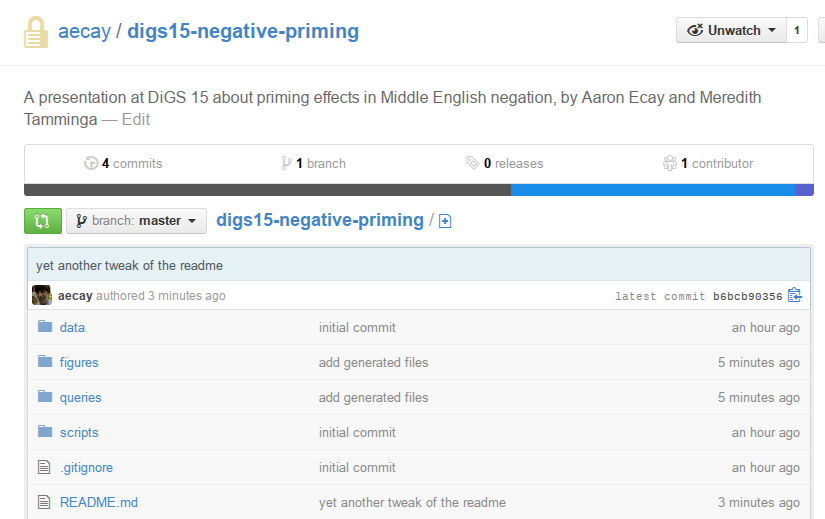
\includegraphics[height=3in]{figures/github}}

\end{frame}

\begin{frame}<beamer>
    \frametitle{Questions}
    \begin{center}
        \Huge
        Questions?
    \end{center}
\end{frame}

\section{Bibliography}
\label{sec:bibliography}

\subsection*{foo}

\begin{frame}[allowframebreaks=0.9]{Bibliography}
    \printbibliography[heading=none]
\end{frame}


\end{document}
